\chapter{Annexes}
\label{chap:annexes}
%\minitoc

\section{Caractéristique d'Euler}

La caractéristique d'Euler, formulée par le mathématicien suisse Leonhard Euler au XVIIIe siècle, joue un rôle central dans les domaines de la topologie et de la géométrie. Elle constitue un outil puissant permettant de décri re de manière élégante et efficace des objets géométriques complexes en utilisant des concepts mathématiques simples. Il s'agit d'un invariant topologique c'est à dire un nombre associé à une variété, qui est invariant par homéomorphisme (c’est-à-dire que la valeur de cet invariant est la même pour deux variétés homéomorphes).

\begin{definition}[\cite{Henri_Paul_de_Saint_Gervais}]
Soit $\Sigma$ une surface compacte. Notons $S$, $A$ et $F$ le nombre de sommets, arêtes et faces d'une décomposition polyédrale de $\Sigma$. Alors le nombre
$$
S-A+F,
$$
est indépendant du choix de cette décomposition polyédrale. On l’appelle caractéristique d’Euler de $\Sigma$ et on la note $\chi(\Sigma)$.
\end{definition}

Nous illustrons cette invariance sur la figure \ref{fig:carre_euler} avec deux triangulation différente d'un même domaine.


\begin{figure}
\begin{subfigure}{0.5\textwidth}
    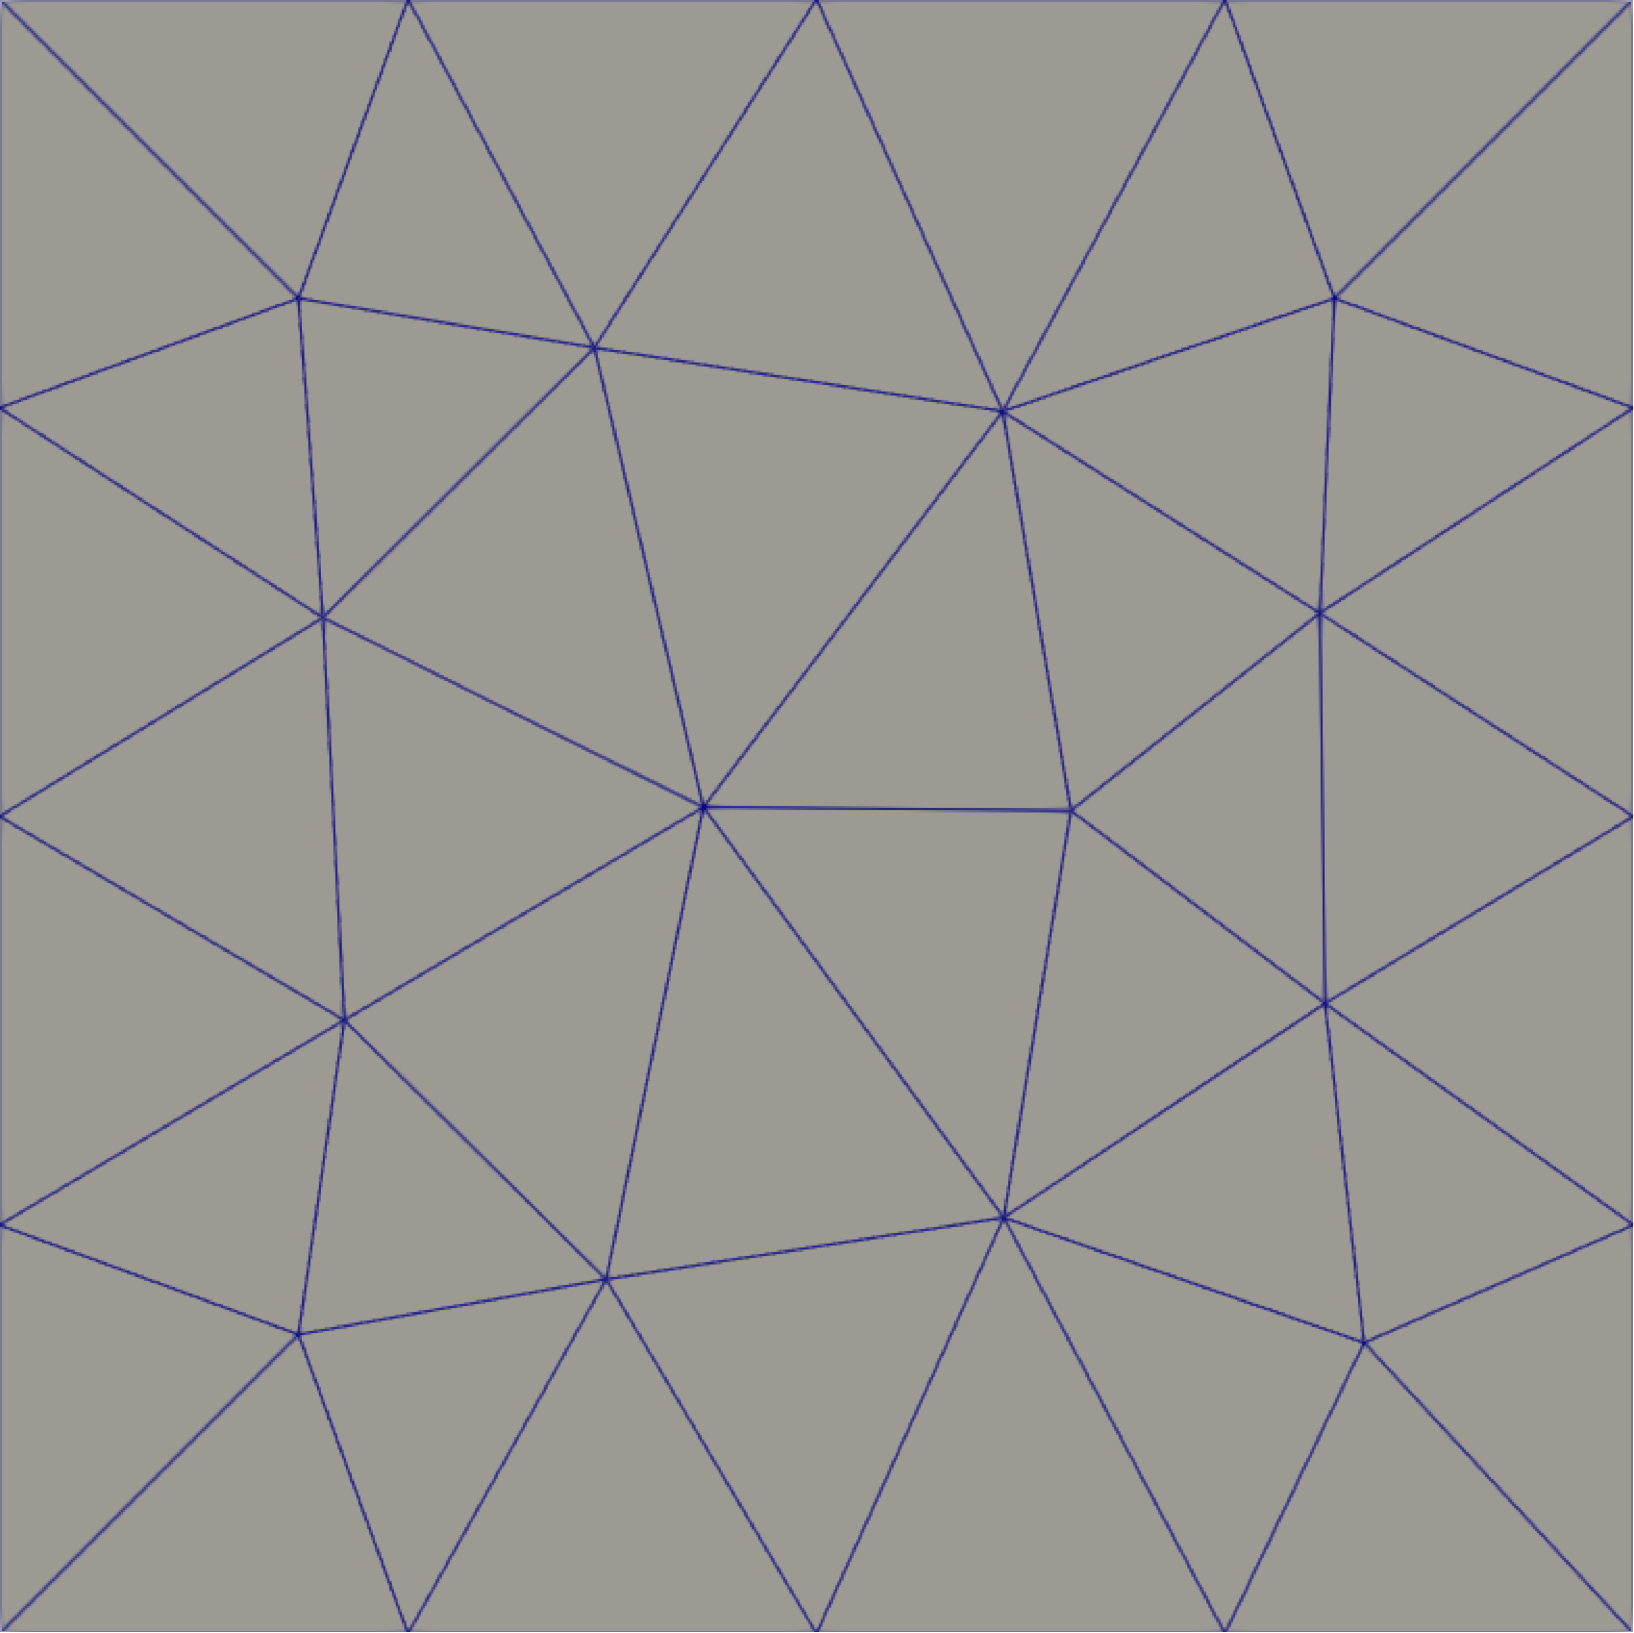
\includegraphics[width=\textwidth]{images/carre_euler_1.pdf}
    %\caption{Maillage triangulaire.}
    %\label{fig:mail_tri_vs_mail_quad_1}
\end{subfigure}
\hfill
\begin{subfigure}{0.5\textwidth}
    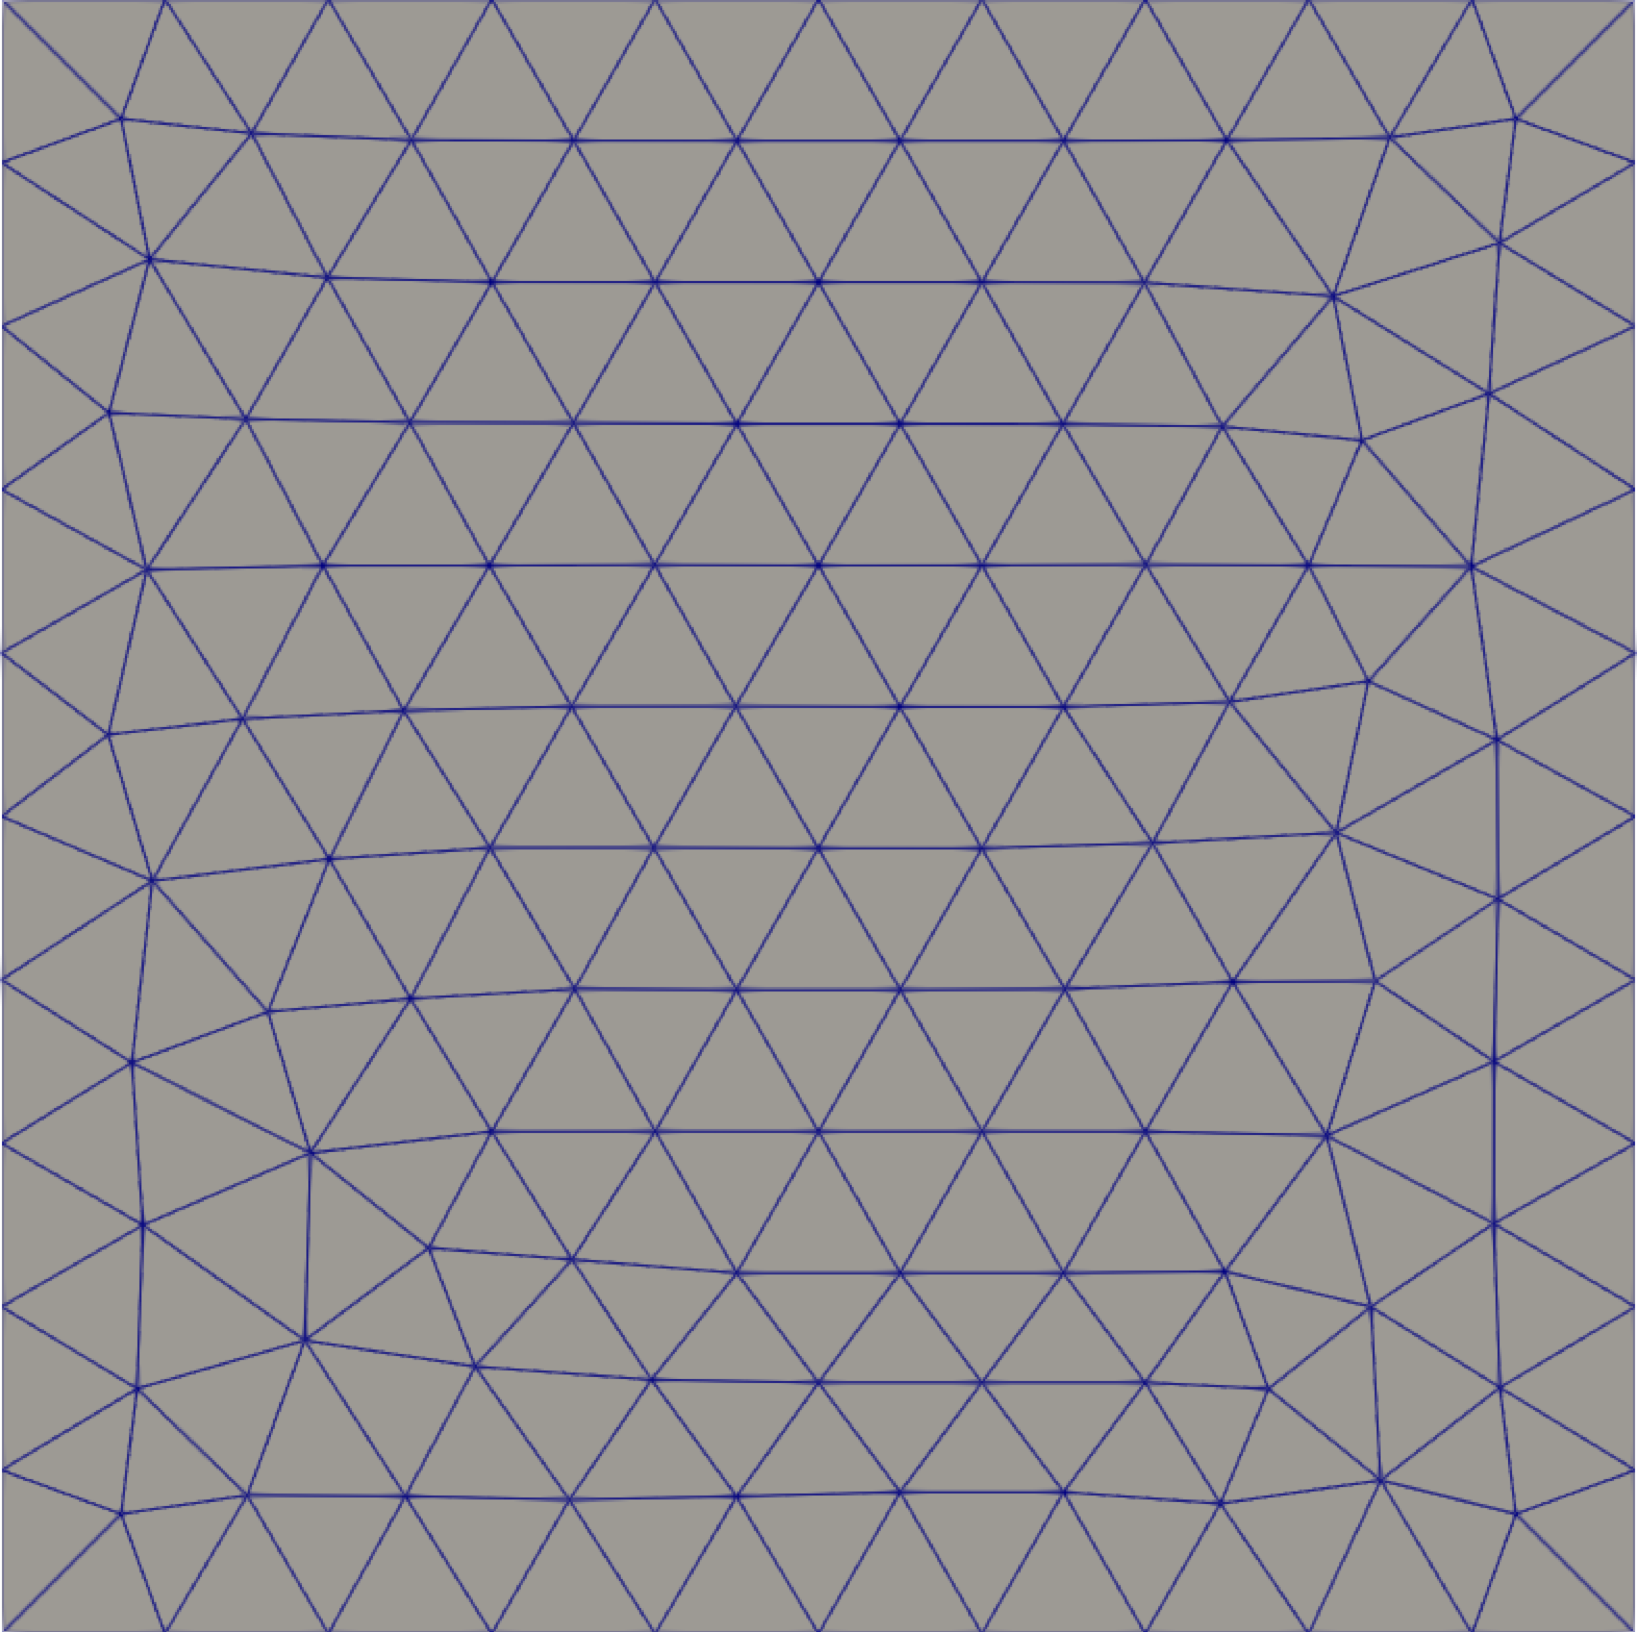
\includegraphics[width=\textwidth]{images/carre_euler_2.pdf}
    %\caption{Maillage quadrilatéral.}
    %\label{fig:mail_tri_vs_mail_quad_2}
\end{subfigure}
\caption{Illustration de l'invariance de la caractéristique d'Euler. A gauche on a une triangulation de 30 sommets, 71 arêtes et 42 triangles et à droite, on a une triangulation de 142 sommets, 383 arêtes et 242 triangles.}
\label{fig:carre_euler}
\end{figure}

La caractéristique d'Euler d'une surface orientable $\Sigma$ peut être calculée à partir de son genre $g$ et du nombre $b$ de composante connexe de son bord:
$$
\chi(\Sigma) = 2-2g-b.
$$

Pour les variétés riemanniennes, la caractéristique d'Euler peut également être trouvée en intégrant la courbure à partir du théorème de Gauss-Bonnet. Ainsi si $\Sigma$ est une variété Riemanienne compact alors on a:

$$
\displaystyle\int_\Sigma KdA+\int_{\partial\Sigma} k_{g}\,ds=2\pi \chi (\Sigma)
$$

Ici, $\partial\Sigma$ désigne le bord de $\Sigma$, $K$ la courbure gaussienne de $\Sigma$ et $k_g$ la courbure géodésique de $\partial\Sigma$. $dA$ est l'élément d'aire de la surface, et $ds$ est l'élément de ligne le long du bord de $\Sigma$.


\section{Opérateur Laplacien discret}

L'opérateur Laplace-Beltrami $\Delta$ occupe une position centrale dans les algorithmes géométriques appliqués aux domaines courbes. La formule des cotangentes, présentée dans \cite{operatorlecture, crane2019n}, offre une approche pratique pour approximer cet opérateur sur des surfaces triangulées bidimensionnelles. Considérons la résolution de l'équation de Poisson
\[ \Delta u = f, \]
sur une surface courbée $\Omega$. Ici, $f : \Omega \rightarrow \mathbb{R}$ représente une fonction source, $u : \Omega \rightarrow \mathbb{R}$ est une fonction inconnue, et $\Delta$ désigne l'opérateur Laplace-Beltrami associé à $\Omega$, également appelé le laplacien. Une méthode courante pour approximer la solution fait appel au concept de solution faible. Les solutions faibles pour l'équation de Poisson sont des fonctions $\phi$ qui satisfont à l'ensemble d'équations suivant :
\[ \int_{\Omega} \phi \Delta u \,dA = \int_{\Omega} \phi f \,dA, \quad \forall \text{ fonctions tests } \phi .\]
Il convient de rappeler que, selon la méthode de Galerkin, le choix des fonctions de base pour $u$, $f$, et la fonction test $\phi$ est essentiel. Ainsi, nous avons besoin d'un ensemble de fonctions de base sur $\Omega$. Pour une surface triangulée, les fonctions chapeau linéaires morceau par morceau $h_i$ se révèlent être le choix le plus naturel. Elles sont définies de manière à valoir un au sommet associé et zéro à tous les autres sommets. Par conséquent, si nous connaissons la valeur de $u(x)$ sur chaque sommet $v_i$, $u(v_i) = u_i$, nous pouvons l'approximer de la manière suivante :
\[ u(x) = \sum_{i} u_ih_i(x) .\]
De même, pour la fonction source $f$, nous avons :
\[ f(x) = \sum_{i} f_ih_i(x). \]
Avec la discrétisation de $u$ et $f$, en utilisant $h_i$ comme fonctions test, nous pouvons maintenant exprimer le problème de Poisson d'origine comme un ensemble de $|V|$ équations :
\[ \int_{\Omega} h_i\Delta u \,dA = \int_{\Omega} h_if \,dA, \quad \forall i \in \{1, 2, . . . , |V|\},\]
où $|V|$ représente le nombre de sommets dans la triangulation.
 Ainsi on a:
\begin{equation}
\left\{
\begin{array}{l}
    \displaystyle\int_{\Omega} h_i\Delta u \,dA = - \int_{\Omega} \nabla h_i \cdot \nabla u \,dA = - \int_{\Omega} \nabla h_i \cdot \nabla \left(\sum_{j} u_j h_j\right) \,dA = - \sum_{j} u_j \int_{\Omega} \nabla h_i \cdot \nabla h_j \,dA,\\\\
    \displaystyle\int_{\Omega} h_if \,dA = \int_{\Omega} h_i \cdot \left(\sum_{j} b_j h_j\right) \,dA = \sum_{j} f_j \int_{\Omega} h_i \cdot h_j \,dA.
\end{array}
\right.
\end{equation}
Soit \(L\) la matrice \(L = \{L_{ij}\}^{|V|\times|V|}\), \(L_{ij} = \displaystyle\int_{\Omega} \nabla h_i \cdot \nabla h_j \,dA\) et \(M\) la matrice \(M = \{M_{ij}\}^{|V|\times|V|}\), \(M_{ij} = \displaystyle\int_{\Omega} h_i \cdot h_j \,dA\). On a alors le problème linéaire:
$$
L\mathbf{u}=M\mathbf{f},
$$
avec
\[
\mathbf{u}=\begin{bmatrix}
u_1\\
u_2\\
\vdots \\
u_{|V|}
\end{bmatrix}
\quad\quad\quad\mbox{ et }\quad\quad\quad
\mathbf{f}=
\begin{bmatrix}
f_1\\
f_2\\
\vdots \\
f_{|V|}
\end{bmatrix}.
\]
Pour calculer la matrice \(L\), nous examinons les éléments \(L_{ij} = \displaystyle\int_{\Omega} \nabla h_i \cdot \nabla h_j \,dA\), dont l'évaluation équivaut au calcul de l'intégrale sur chaque triangle, suivi de la sommation des résultats obtenus sur l'ensemble des triangles de \(\Omega\). Étant donné que \(h_i\) est une fonction linéaire par morceau sur chaque triangle, le calcul sur un triangle donné revient à multiplier le scalaire \(\nabla h_i \cdot \nabla h_j\) sur ce triangle par la surface du triangle. Nous allons maintenant examiner le gradient d'une fonction linéaire sur un triangle.

Soit $g$ une fonction linéaire définie sur un triangle $T$ de sommets $v_1$, $v_2$, $v_3$ et d'aire $A$ avec \(g(v_1) = 1\), \(g(v_2) = g(v_3) = 0\). $g$ étant linéaire, on a \(g(x) = g(x_0) + \nabla g |_{x_0} \cdot (x - x_0)\) pour tout $x$ appartenant au triangle.
Sachant que \(\nabla g \cdot (v_1 - v_3) = 1\) et \(\nabla g \cdot (v_2 - v_3) = 0\), il vient que \(\nabla g\) est perpendiculaire à l'arête \(v_2v_3\) et on a d'une part:
\[
||\nabla g|| \|\overrightarrow{v_1v_3}\| \cos\left(\displaystyle\frac{\pi}{2} - \theta_3^{12}\right) = ||\nabla g|| \|\overrightarrow{v_1v_3}\| \sin \theta_3^{12}=1,
\]
autrement dit,
\[
||\nabla g||=\frac{1}{h},
\]
et d'autre part:
\[\nabla g= \displaystyle\frac{\overrightarrow{v_2v_3}^\perp}{2A}\mbox{ puisque } A=\displaystyle\frac{1}{2} \|\overrightarrow{v_2v_3}\|h,
\]
où $h$ est la hauteur passant par $v_1$ et perpendiculaire au côté $v_2v_3$ avec \(\overrightarrow{v_2v_3}^\perp\) la rotation dans le sens anti-horaire de \(\overrightarrow{v_2v_3}\) d'angle \(\pi/4\). Ainsi lorsqu'on a deux fonction définit sur le même sommet, on a:
\[
\begin{array}{lcl}
\displaystyle\int_T \langle \nabla g, \nabla g \rangle dT &= &A||\nabla g||^2\\\\
&=& A\displaystyle\frac{1}{h^2} \\\\
&=& \displaystyle\frac{b}{2h}
\end{array}
\]
où $h$ désigne la hauteur passant par le sommet en question et $b$ est la longueur du côté opposé à ce sommet. En notant $\alpha$ et $\beta$ les angles intérieurs aux deux autres sommets du triangle, on se retrouve alors avec la formule:
\[
\begin{array}{lcl}
\displaystyle\int_T \langle \nabla g, \nabla g \rangle dT  &=& \displaystyle\frac{h \cot \alpha + h \cot \beta}{2h}\\\\
&=& \displaystyle\frac{1}{2} (\cot \alpha + \cot \beta)
\end{array}
\]
Regardons maintenant le cas où les deux fonctions sont définies sur des sommets différents mais de la même arête. Soit $v_2$ et $v_3$ ces sommets. On note $h$ la hauteur passant par le sommet $v_1$ et perpendiculaire à l'arête $v_2v_3$ et on note $b$ la longeur de cette arête. On a:
\[
\begin{array}{lcl}
\displaystyle\int_T \langle \nabla g_2, \nabla g_3 \rangle dT &= &A\langle \nabla f_2, \nabla f_3 \rangle\\\\
&=& \displaystyle\frac{1}{4A} \langle \overrightarrow{v_3v_1}^\perp, \overrightarrow{v_1v_2}^\perp \rangle\\\\
&=& -\displaystyle\frac{\|\overrightarrow{v_3v_1}\|\|\overrightarrow{v_1v_2}\| \cos \theta_1^{23}}{4A}\\\\
&=& -\displaystyle\frac{(h/\sin \theta_2^{31})(h/\sin \theta_3^{12}) \cos \theta_1^{23}}{2bh}\\\\
&=& -\displaystyle\frac{h \cos \theta_1^{23}}{2(h \cot \theta_2^{31} + h \cot \theta_3^{12}) \sin \theta_2^{31} \sin \theta_3^{12}}\\\\
&=& -\displaystyle\frac{\cos \theta_1^{23}}{2(\cos \theta_2^{31} \sin \theta_3^{12} + \cos \theta_3^{12} \sin \theta_2^{31})}\\\\
&=& -\displaystyle\frac{\cos \theta_1^{23}}{2 \sin(\theta_2^{31} + \theta_3^{12})}\\\\
&=& -\displaystyle\frac{\cos \theta_1^{23}}{2 \sin \theta_1^{23}}\\\\
\displaystyle\int_T \langle \nabla f_2, \nabla f_3 \rangle dT&=& -\displaystyle\frac{1}{2 \cot \theta_1^{23}}
\end{array}
\]
En appliquant ces résultats sur les fonctions chapeau \(h_i\) avec les notations de la figure  , on obtient:

\[
\langle \nabla h_p, \nabla h_p \rangle = \frac{1}{2} \sum_i (\cot \alpha_i + \cot \beta_i)
\]
\[
\langle \nabla h_p, \nabla h_q \rangle = -\frac{1}{2} (\cot \theta_1 + \cot \theta_2)
\]
Enfin, nous obtenons la matrice laplacienne cotangente \(L\):

\[
L_{ij} =
\begin{cases}
\displaystyle\frac{1}{2} \sum_{i\sim j} (\cot \alpha_j + \cot \beta_j), & \text{si } i = j, \\\\
-\displaystyle\frac{1}{2} (\cot \alpha_j + \cot \beta_j), & \text{si } i \neq j, \\\\
0, & \text{sinon}.
\end{cases}
\]


%theoreme des tangentes tournantes
%Algorithme glouton pour le partitionnement en sous maillage
